\section{Convolutional Neural Networks}  
This is the fourth course of deep learning specialization at Coursera taught by Professor Andrew Ng. Here is my certificate after finishing this course (Fig. \ref{C4-Certificate}):

\begin{figure}[!htbp]
    \centering
    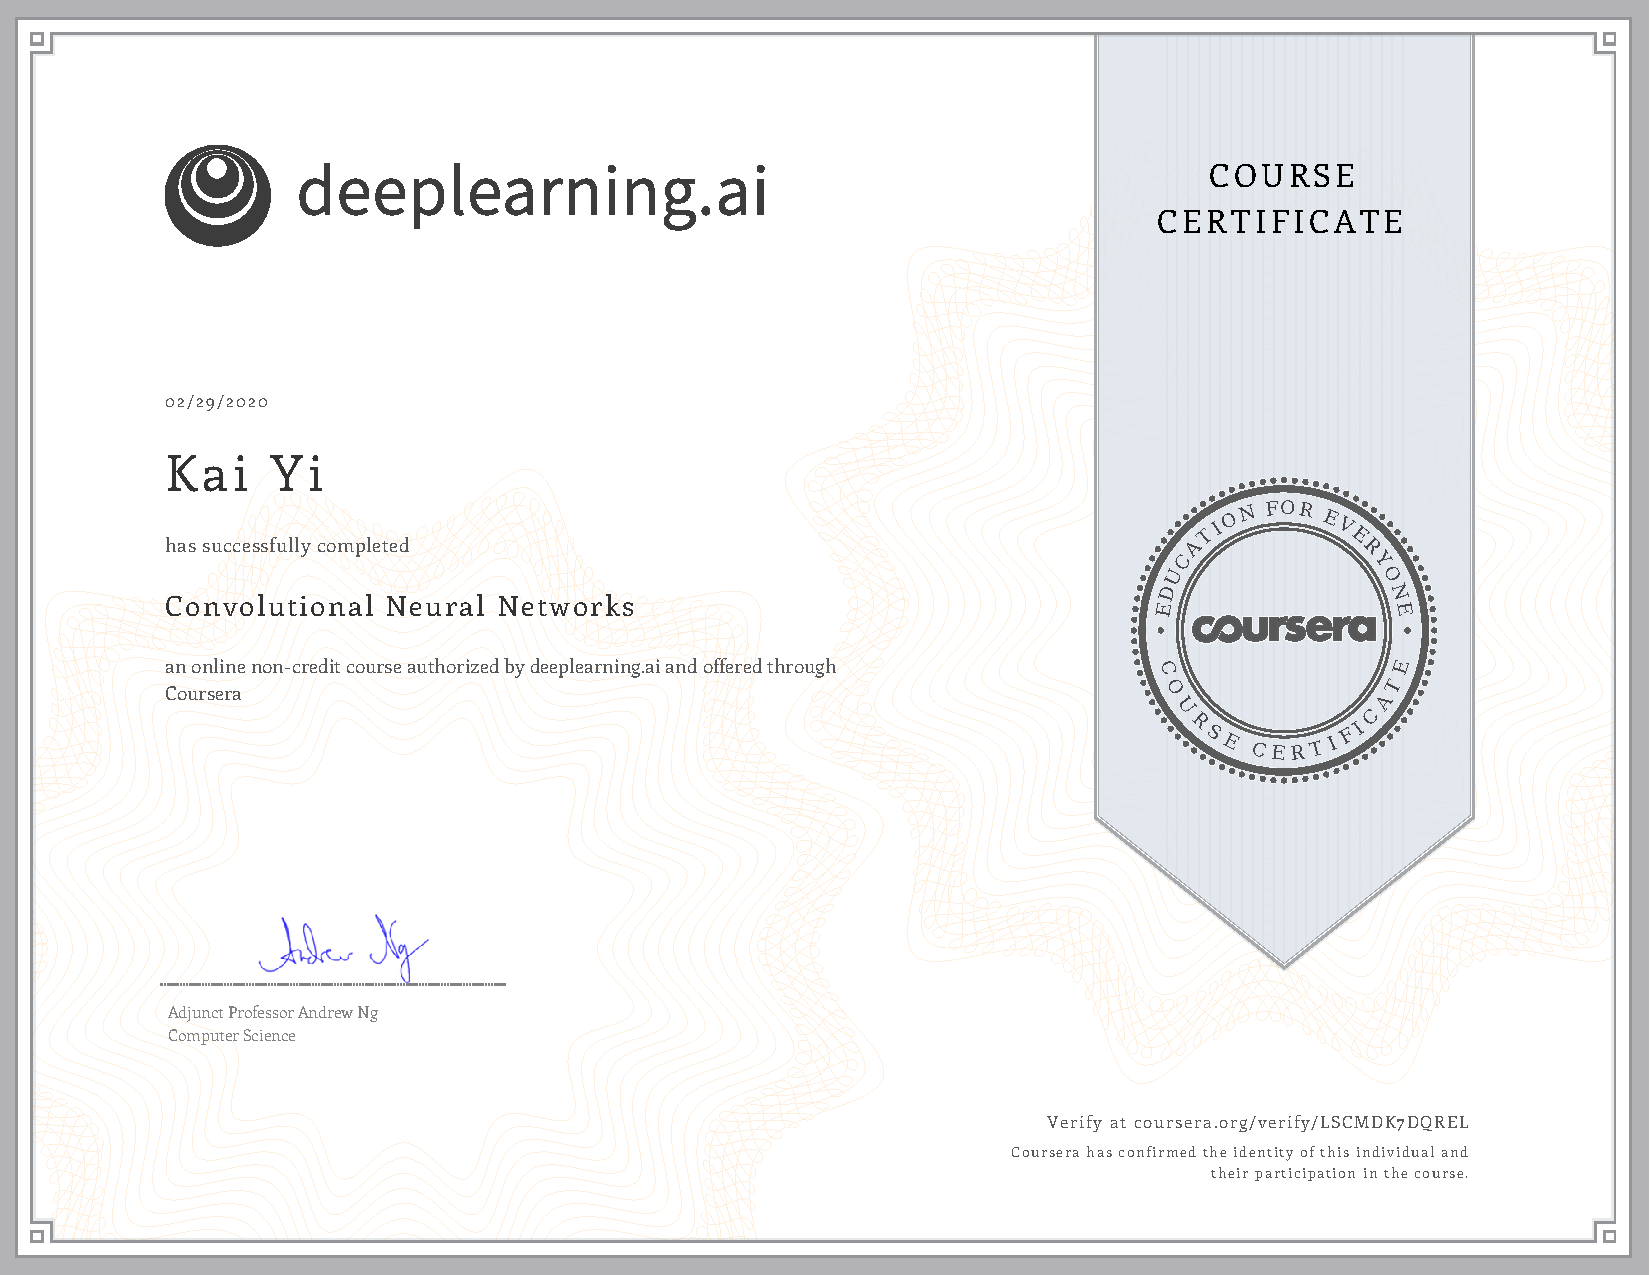
\includegraphics[width=1.0\textwidth]{img/C4-Certificate.pdf}
    \caption{Certificate of Convolutional Neural Networks. Obtained in Feb. 2020.}
    \label{C4-Certificate}
\end{figure}

\subsection{Course Overview}
According to the official site of this course, there are following key components:

\begin{itemize}
    \item Understand how to build a convolutional neural network, including recent variations such as residual networks.
    \item Know how to apply convolutional networks to visual detection and recognition tasks.
    \item Know to use neural style transfer to generate art.
    \item Be able to apply these algorithms to a variety of image, video, and other 2D or 3D data.
\end{itemize}

\subsection{Foundations of CNNs}
The aims of this section is to implement the foundational layers of CNNs (pooling, convolutions) and to stack them properly in a deep network to solve multi-class image classification problems.

\subsubsection{Edge Detection Example}
Early layers of CNN might detect edges then the middle layers will detect parts of objects and the later layers will put these parts together to produce an output.

\subsubsection{Padding, Stride}
\begin{equation}
    C_{out} = (C_{in} - k + 2*p) / s + 1
\end{equation}

k represents the kernel size, p represents padding and s represents stride.

\subsubsection{Pooling layers}
Other than the conv layers, CNNs often uses pooling layers to reduce the size of the inputs, speed up computation, and to make some of the features it detects more robust.

The max pooling is saying, if the feature is detected anywhere in this filter then keep a high number. But the main reason why people are using pooling because its works well in practice and reduce computations.

Max pooling has no parameters to learn.

Average pooling is taking the averages of the values instead of taking the max values.

Max pooling is used more often than average pooling in practice.

If stride of pooling equals the size, it will then apply the effect of shrinking.

\subsubsection{Convolutional Neural Network Example}
Here are some statistics about a mentioned example (Fig. \ref{cnn-example}):

\begin{figure}[!htbp]
    \centering
    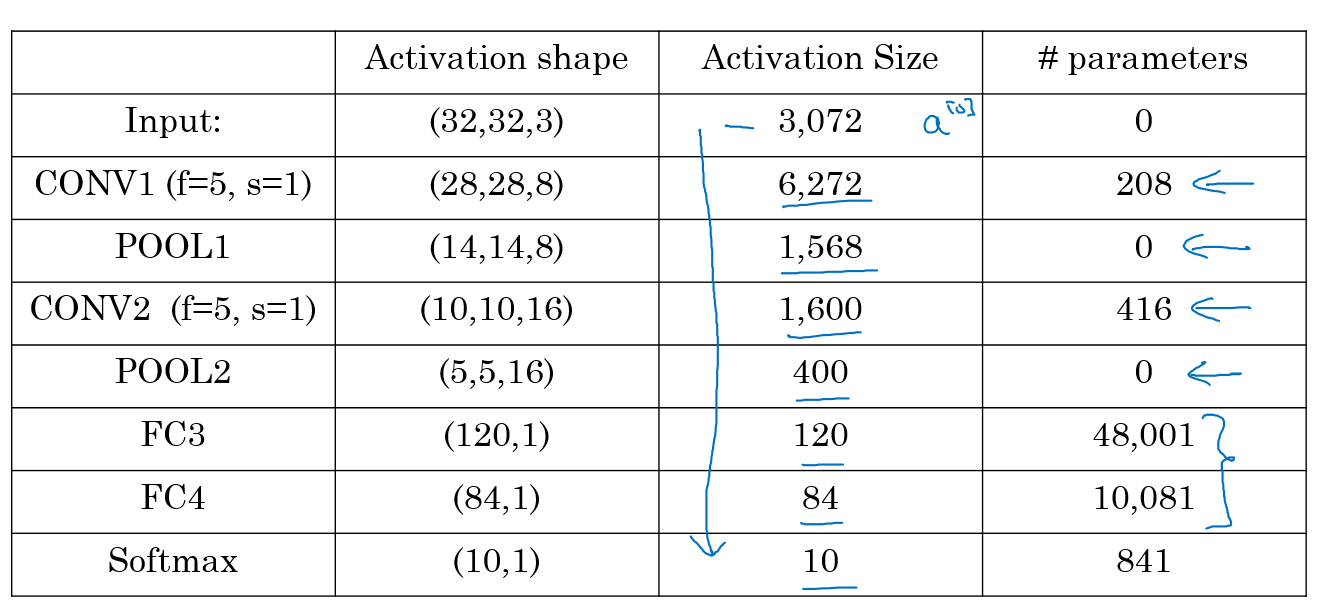
\includegraphics[width=1.0\textwidth]{img/c4/cnn-examples.png}
    \caption{Some statistics about a LeNet-like network. Every parameter is calculated by $(k^2+1)*c$, k represents kernel size and c represents output channel.}
    \label{cnn-example}
\end{figure}

Usually the input size decreases over layers which the number of filters increases.

A CNN usually consists of one or more convolution (not just one as the shown example) followed by a pooling.

Fully connected layers has the most parameters in the network.

\subsubsection{Why Convolutions?}
Two main advantages of Convs are:

\begin{itemize}
    \item Parameter sharing. A feature detector (such as a vertical edge detector) that's useful in one part of the image is probably useful in another part of the image.
    \item Sparsity of Connections. In each layer, each output value depends only on a small number of inputs which makes it translation invariance (Translation invariance means that the system produces exactly the same response, regardless of how its input is shifted.).
\end{itemize}

\subsection{Deep Convolutional Models: Case Studies}
The goal of this section is to learn about the practical tricks and methods used in deep CNNs straight from the research papers.

\subsubsection{Classic Networks}
In this subsection we will talk about classic networks which are LeNet-5, AlexNet and VGG.

\paragraph{LeNet-5} The goal for this model was to identify handwritten digits in a $32\times 32\times 1$ gray image. Here is the drawing of it (Fig. \ref{lenet}):

\begin{figure}[!htbp]
    \centering
    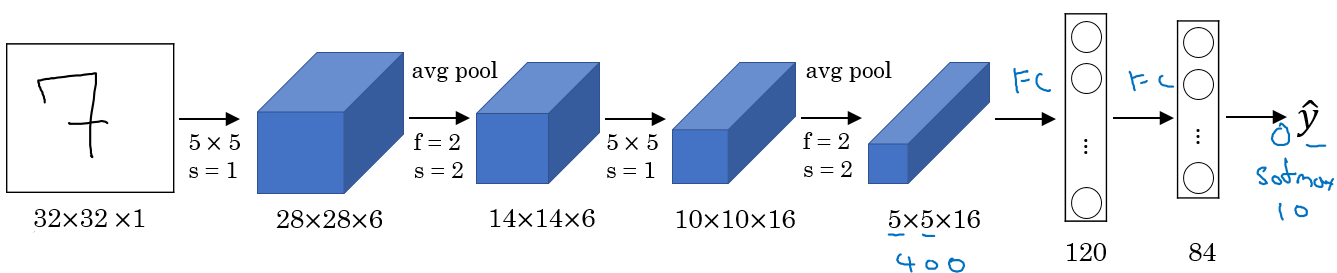
\includegraphics[width=1.0\textwidth]{img/c4/lenet.png}
    \caption{LeNet architecture.}
    \label{lenet}
\end{figure}

This model was published in 1998 \cite{lecun1998gradient}. The last layer wasn't using softmax back then.

It has 60k parameters.

The dimensions of the image decreases as the number of channels increases.

$Conv \to Pool \to Conv \to Pool \to FC \to FC \to Softmax$ this type of arrangement is quite common.

The activation function used in the paper was Sigmoid and Tanh. Modern implementation uses ReLU in most of the cases.

\paragraph{AlexNet} Named after Alex Krizhevsky who was the first author of this paper \cite{krizhevsky2012imagenet}. The other authors includes Geoffrey Hinton.

The goal for this model was the ImageNet challenge which classifies images into 1000 classes. Here are the drawing of this model:

\begin{figure}[!htbp]
    \centering
    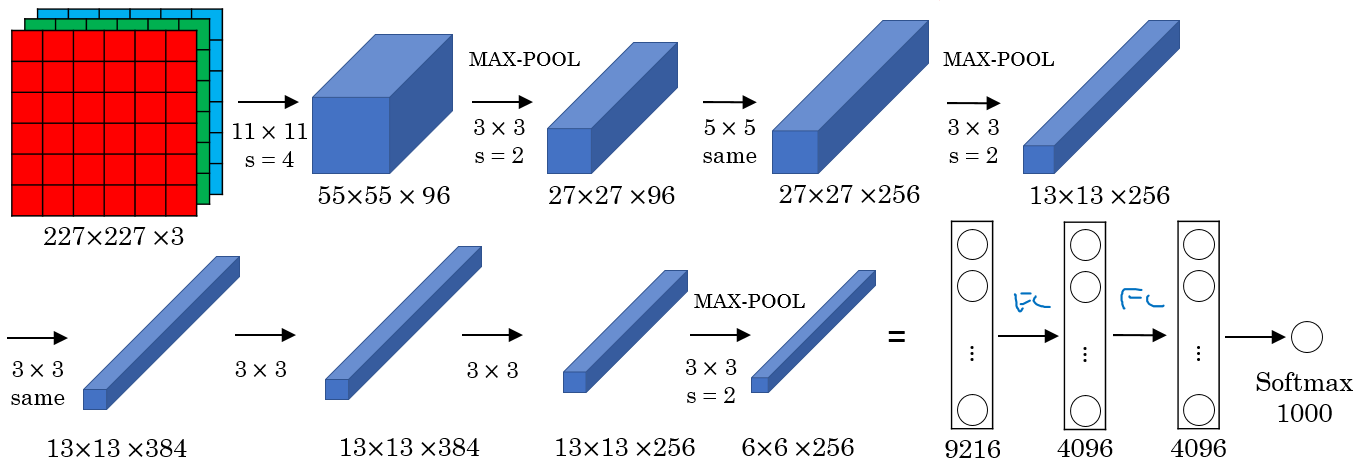
\includegraphics[width=1.0\textwidth]{img/c4/alexnet.png}
    \caption{AlexNet architecture.}
    \label{lenet}
\end{figure}

Architecture:

$Conv \to Max-pool\to Conv\to Max-pool\to Conv\to Conv\to Conv\to Max-pool\to Flatten\to FC\to FC\to Softmax$

Similar to LeNet-5 but bigger.

Has 60 million parameters compared to 60k parameterof LeNet-5.

It used the ReLU activation function.

The original paper contains multiple GPUs and Local Response Normalization (LRN). Multiply GPUs were used because the GPUs were not so fast back then. Researchers proved that LRN doesn't help much so for now don't botter yourself for understanding or implementing it.

This paper convinced the computer vision researchers that deep learning is so important.

\paragraph{VGG-16} VGG-16 \cite{simonyan2014very} is a modification fro AlexNet.

Instead of having a lot of hyperparameters let's have some simpler network.

Focus on having only these blocks:
\begin{itemize}
    \item Conv = $3\times 3$, filter, s = 1, 'SAME'
    \item Max-Pool = $2\times 2$, s = 2
\end{itemize}

Here is the architecture (Fig. \ref{vgg16}):

\begin{figure}[!htbp]
    \centering
    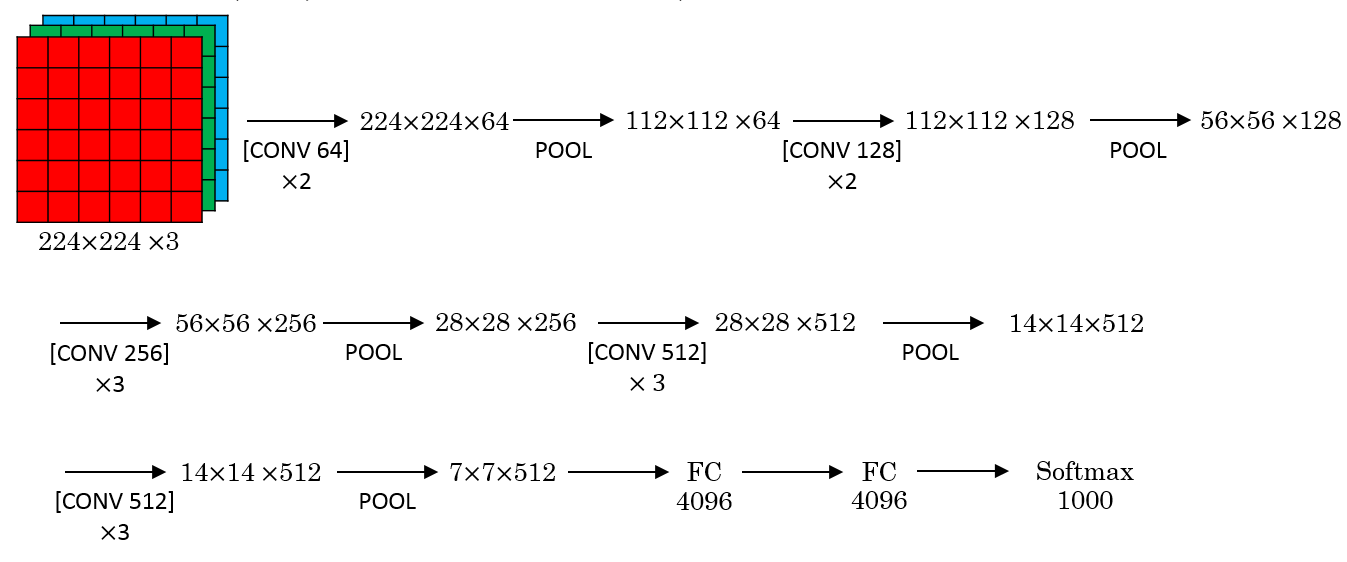
\includegraphics[width=1.0\textwidth]{img/c4/vgg16.png}
    \caption{VGG-16 architecture.}
    \label{vgg16}
\end{figure}

This network is large even by modern standards. It has around 138 million parameters (Most of the parameters are in the fully connected layers).

In has a total memory of 96MB per image for only forward propagation (Most memory are in the earlier layers).

Number of filers increases from 64 to 128 to 256 to 512. 512 was made twice.

Pooling was the only one who is responsible for shrinking the dimensions.

There are another version called VGG-19 which is a bigger version. But most people uses the VGG-16 instead of the VGG-19 because it does the same.

VGG paper is attractive it tries to make some rules regarding using CNNs.

\subsubsection{Residual Networks (ResNets)}
Very, very deep NNs are difficult to train becaus of vanishing and exploding gradiednts problems.

In this section we will learn about skip connection which makes you take the activation from one layer and subsequently feed it to another layer even much deeper in NN which allows you to train large NNs even with layers greater than 100.

\paragraph{Residual Block}
ResNets are built out of some Residual blocks (Fig. \ref{resblock}).

\begin{figure}[!htbp]
    \centering
    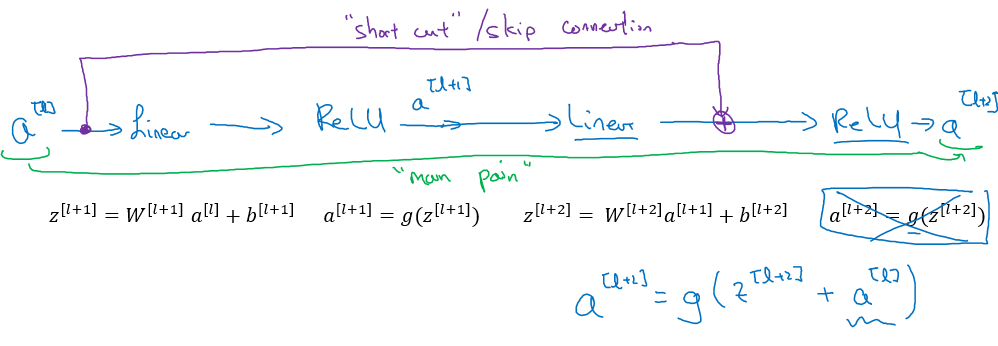
\includegraphics[width=1.0\textwidth]{img/c4/resblock.png}
    \caption{Residual block architecture.}
    \label{resblock}
\end{figure}

They add a shortcut/skip connection before the second activation.

The authors of this block find that you can train a deeper NNs by stacking this block.

\paragraph{Residual Network}
Are a NN that consists of some Residual blocks (Fig. \ref{resnet}).

\begin{figure}[!htbp]
    \centering
    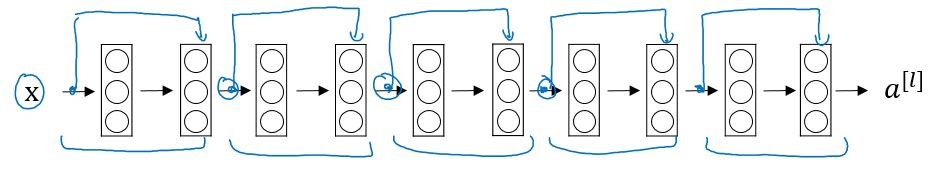
\includegraphics[width=1.0\textwidth]{img/c4/resnet.png}
    \caption{Residual network architecture.}
    \label{resnet}
\end{figure}

These networks can go deeper without hurting the performance. In the normal NN - Plain networks - the theory tell us that if we go deeper we will get a better solution to out problem, but because of the vanishing and exploding gradients problems the performances of the network suffers as it goes deeper. Thanks to Residual Network we can go deeper as we want now (Fig. \ref{plain-vs-resnet}).

\begin{figure}[!htbp]
    \centering
    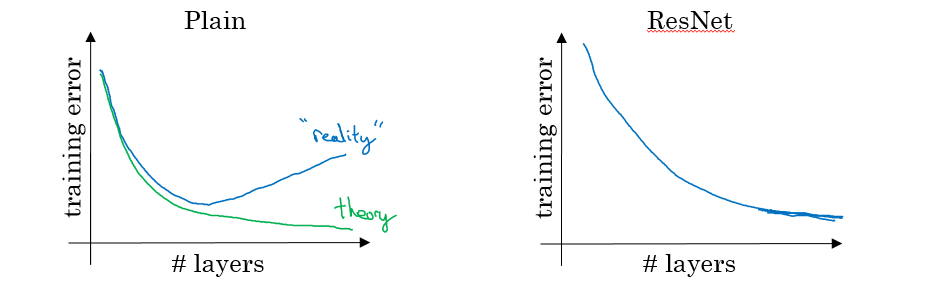
\includegraphics[width=1.0\textwidth]{img/c4/plain-vs-resnet.png}
    \caption{Plain networks vs. ResNet}
    \label{plain-vs-resnet}
\end{figure}

On the left is the normal NN and on the right are the ResNet. As you can see the performance of ResNet increases as the network goes deeper.

In some cases going deeper won't effect the performance and that depends on the problem on your hand.

Some people are trying to train 1000 layer now which isn't used in practice.

\subsubsection{Why ResNets Work}
Lets see some example that illustrates why ResNets work.

We have a big NN as the following: $X \to Big\ NN\to a[l]$.

Lets add two layers to this network as a residual block: $X \to Big\ NN\to a[l] \to layer1 \to layer2\to a[i+2]$. $a[i]$ has a direct connection to $a[i+2]$.

Suppose we are using ReLU activations.

Then:

\begin{lstlisting}
a[l+2] = g(z[l+2] + a[l])
       = g(W[l+2] a[l+1] + b[l+2] + a[l])
\end{lstlisting}

Then if we are using L2 regularization as an example,  Let's say $W[l+2]$ and $b[l+2]$ will be zero. Then $a[l+2]=g(a[l]) = a[l]$ with no negative values.

This show that identity function function is easy for a residual block to learn. And that's why it can train deeper NNs.

Also that the two layers we added doesn't hurt the performance of big NN we made.

Hint: dimensions of z[l+2] and a[l] have to be the same in resNets. In case they have different dimensions what we put a matrix parameters (Which can be learned or fixed)

\begin{itemize}
    \item $a[l+2] = g( z[l+2] + ws * a[l] )$ \# The added Ws should make the dimensions equal.
    \item ws also can be a zero padding.
\end{itemize}

Using a skip-connection helps the gradient to backpropagate and thus helps you to train deeper networks.

Lets take a look at ResNet on images. Here is the architecture of ResNet-34 (Fig. \ref{resnet-34}):

\begin{figure}[!htbp]
    \centering
    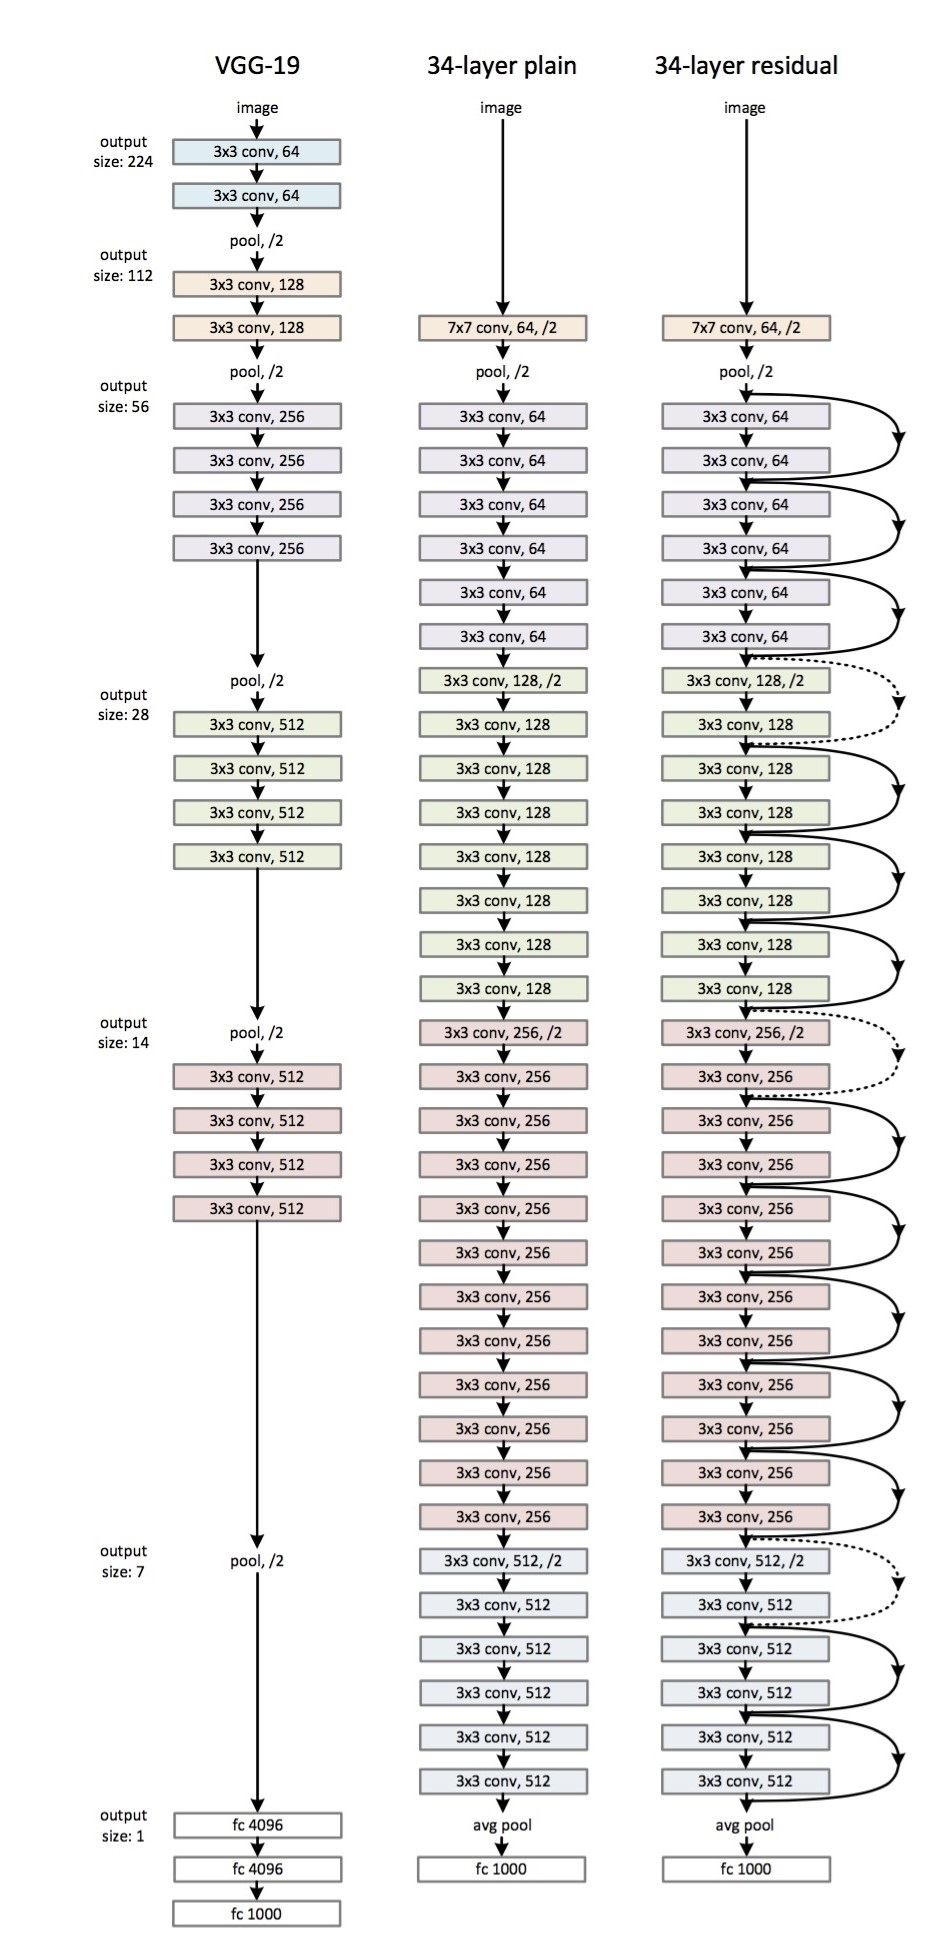
\includegraphics[width=1.0\textwidth, height=1.3\textwidth]{img/c4/resnet-34.jpg}
    \caption{ResNet-34 compared with VGG-19 and 34-layer plain network.}
    \label{resnet-34}
\end{figure}

In ResNet-34:

\begin{itemize}
    \item All the $3\times 3$ Conv are same Convs.
    \item Keep it simple in design of the network.
    \item Spatial Size / 2 $\to$ Number of filters * 2.
    \item No FC layers, no dropout is used.
    \item Two main types of blocks are used in a ResNet, depending mainly on whether the input/output dimensions are same or different. You are going to implement both of them.
    \item The dotted lines is the case when the dimensions are different. To solve then they down-sample the input by 2 and then pad zeros to match the two dimensions. There's another trick which is called bottleneck which we will explore later.
\end{itemize}

\subsubsection{Residual Block Types}
\paragraph{Identity Block}
Here is the identity block (Fig. \ref{identity-block}):

\begin{figure}[!htbp]
    \centering
    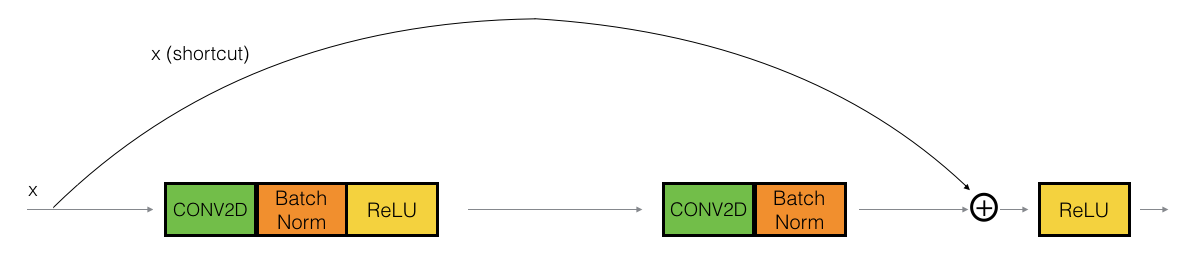
\includegraphics[width=1.0\textwidth]{img/c4/identity-block.png}
    \caption{Identity block.}
    \label{identity-block}
\end{figure}

The Conv is followed by a batch norm before ReLU. Dimensions here are same.

This skip is over 2 layers. The skip connection can jump n connections where n>2.

\paragraph{Convolutional Block} Here is the convolutional block (Fig. \ref{convolutional-block}):

\begin{figure}[!htbp]
    \centering
    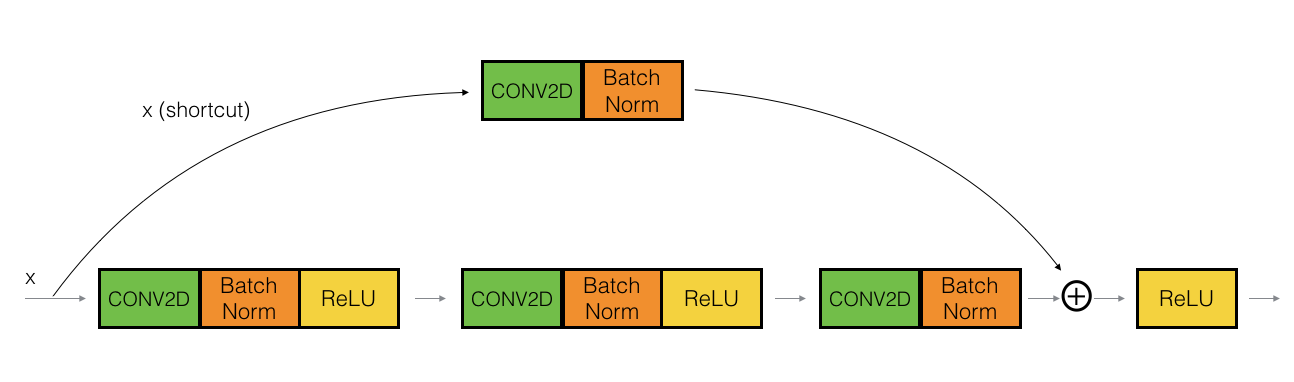
\includegraphics[width=1.0\textwidth]{img/c4/conv-block.png}
    \caption{Convolutional block.}
    \label{convolutional-block}
\end{figure}

The Conv can be bottleneck $1\times 1$ Conv.

\subsubsection{Network in Network and 1 Times 1 Convolutions}
A $1\times 1$ convolution - a very important operation in Network in Network \cite{lin2013network}- is very useful in many CNN modes.

A $1\times 1$ convlution is useful when: 
\begin{itemize}
    \item We want to shrink the number of channels. We also call this feature transformation.
    \item Save computations.
    \item If we have specified the number of 1 x 1 Conv filters to be the same as the input number of channels then the output will contain the same number of channels. Then the 1 x 1 Conv will act like a non linearity and will learn non linearity operator.
\end{itemize}

\subsubsection{Inception Network Motivation}
When you design a CNN you have to decide all the layers yourself. You may pick a $3\times 3$ Conv or $5\times 5$ Conv or maybe a max pooling layer. You have so many choices.

What \textbf{Inception} tell us is, why not use all of them at one?

Inception module \cite{szegedy2015going}, naive version (Fig. \ref{inception-naive}):

\begin{figure}[!htbp]
    \centering
    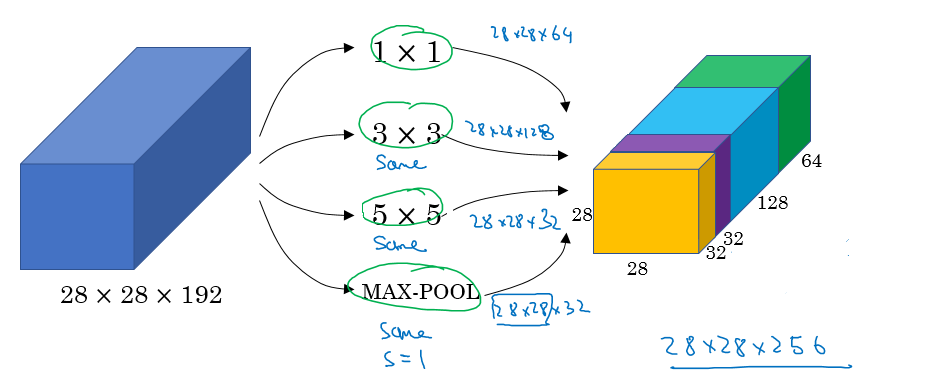
\includegraphics[width=1.0\textwidth]{img/c4/inception-naive.png}
    \caption{Inception module, naive version.}
    \label{inception-naive}
\end{figure}

Max-pool is 'SAME' here.

Input to the inception module is $28\times 28\times 192$ and the output is $28\times 28\times 256$.

We have done all the Convs and pools we might want and will let the NN learn and decide which it want to use most.

% The problem of computational cost in Inception model:

% \begin{itemize}
%     \item 
% \end{itemize}

There is high computational cost in Inception model especially for convolution operations with big kernel size. However, we can use $1\times 1$ convolution to reduce the total number of multiplications.

A $1\times 1$ Conv here is called Bottleneck. It turns out that $1\times 1$ Conv won't hurt the performance.

Inception module, dimensions reduction version (Fig. \ref{inception-reduced}):

\begin{figure}[!htbp]
    \centering
    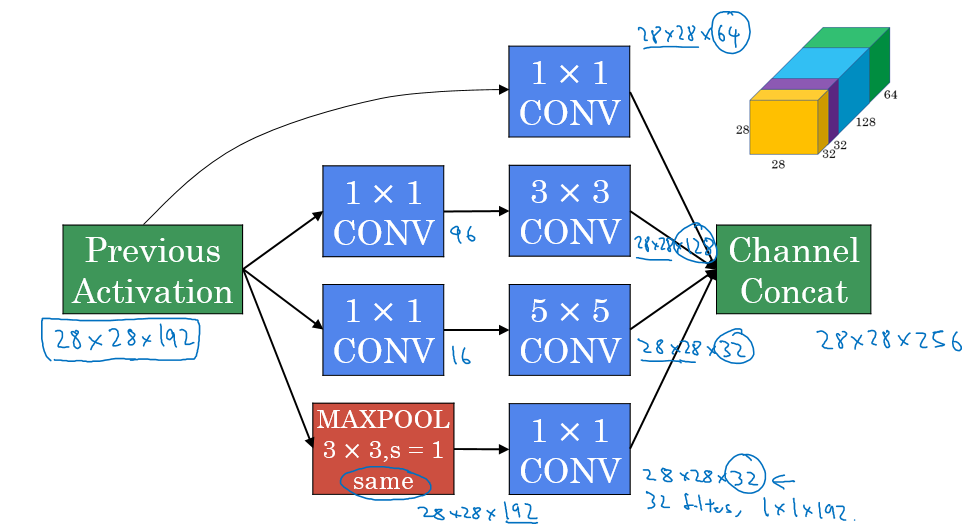
\includegraphics[width=0.9\textwidth]{img/c4/inception-reduced.png}
    \caption{Inception module, dimensions reduction version.}
    \label{inception-reduced}
\end{figure}

Example of inception model in Keras (Figure \ref{inception-keras}):

\begin{figure}[!htbp]
    \centering 
    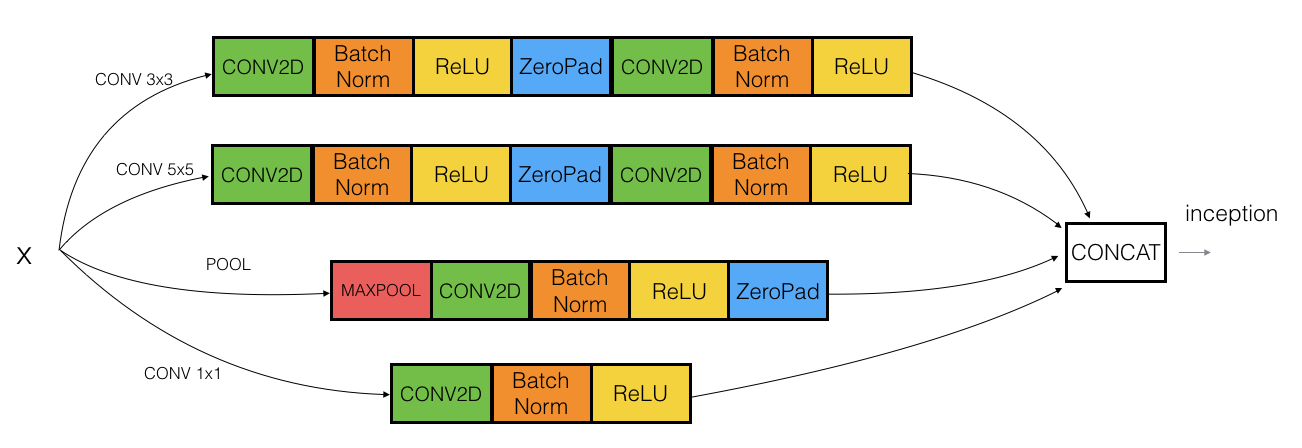
\includegraphics[width=1.0\textwidth]{img/c4/inception_keras.png}
    \caption{Inception module in Keras}
    \label{inception-keras}
\end{figure}

\subsubsection{Inception Network (GoogLeNet)}
The inception network consist of concatenated blocks of the Inception module.

The full model of GoogLeNet \cite{szegedy2015going} can be found at \href{https://nbviewer.jupyter.org/github/mbadry1/DeepLearning.ai-Summary/blob/master/4-\%20Convolutional\%20Neural\%20Networks/Images/15.png}{Here} (Also Figure \ref{googlenet}):

% Replace it with a new url.

\begin{figure}[!htbp]
    \centering 
    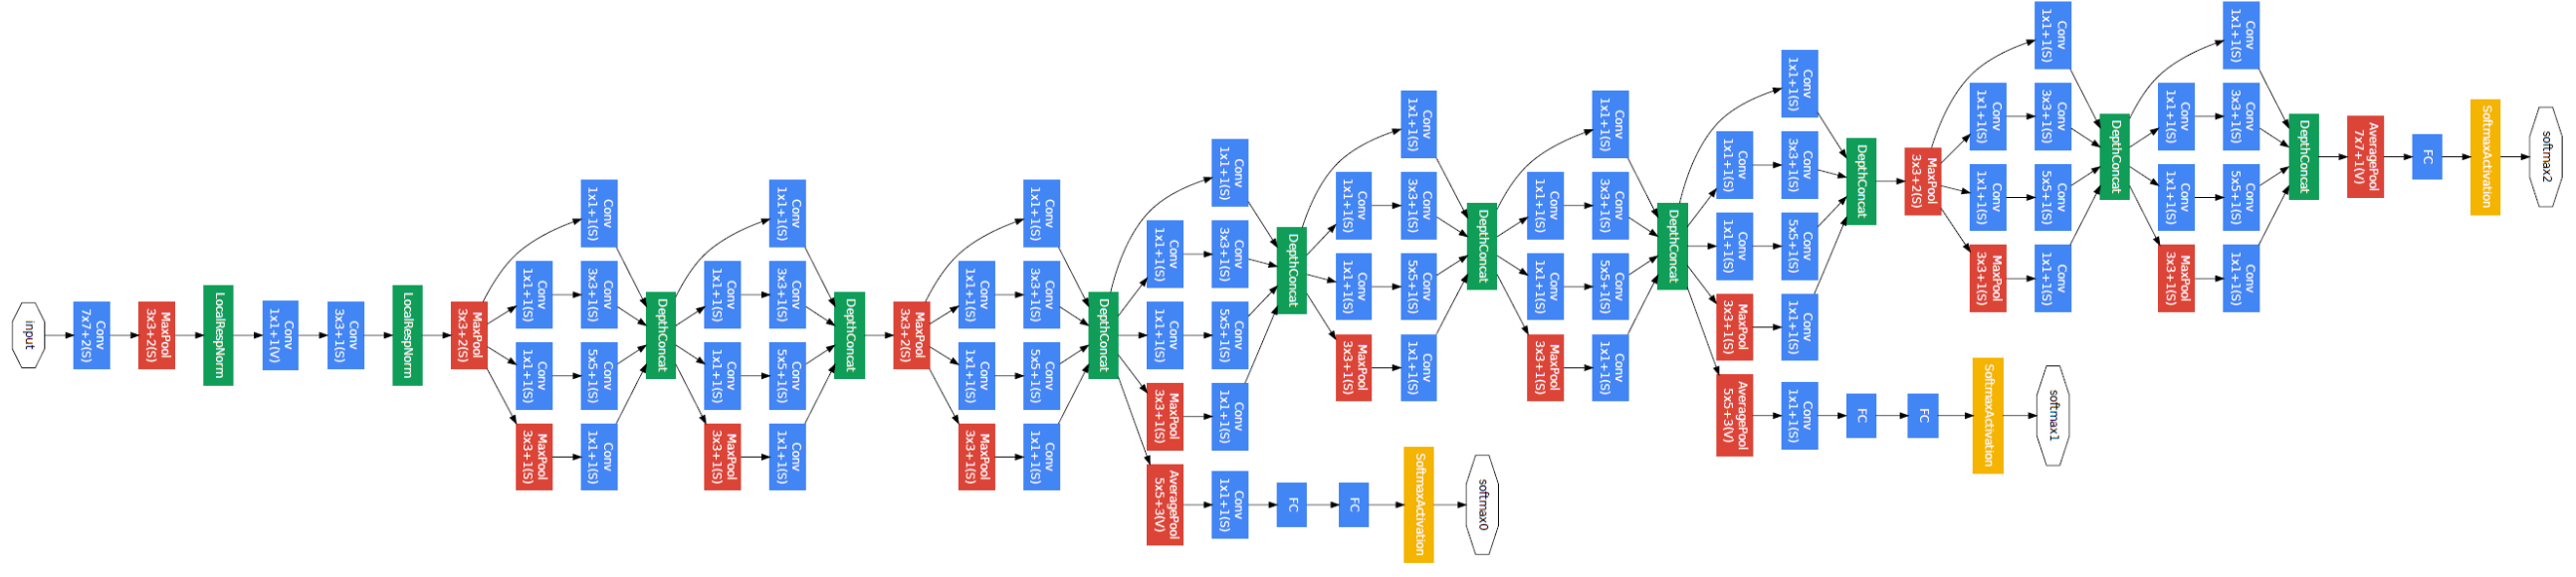
\includegraphics[width=1.1\textwidth, trim={0 0 0 0}, clip]{img/c4/google-net2.png}
    \caption{GoogLeNet architecture.}
    \label{googlenet}
\end{figure}

Some times a max-pool block is used before the inception module to reduce the dimensions of the inputs.

There are 3 softmax branches at different positions to push the network toward its goal, and helps to ensure that the intermediate features are good enough to the network and it turns out that softmax0 and softmax1 gives regularization effect.

Since the development of the Inception module, the authors and the others have built another versions of this network. Like inception v2, v3, and v4. Also there is a network that has used the inception module and the ResNet together.

\subsubsection{Transfer Learning}
If you're using a specific NN architecture that has been trained before, you can use this pretained parameters/weights instead of random initialization to solve your problem.

It can help you boost the performance of the NN.

The pretrained models might have trained on a large dataset like ImageNet or COCO and took a lot of time to learn those parameters/weights with optimized hyperparameters. This can save you a lot of time (parameters freezing technique).

\subsubsection{Data Augmentation}
If data is increased, your deep NN will perform better. Data augmentation is one of the technique that deep learning uses to increase the performance of deep NN.

The majority of computer vision applications needs more data right now.

Some data augmentation methods that are used for computer vision tasks includes:

\begin{itemize}
    \item Mirroring.
    \item Random cropping.
    \begin{itemize}
        \item The issue with this technique is that you might take a wrong crop.
        \item The solution is to make your crops big enough.
    \end{itemize}
    \item Rotation.
    \item Shearing.
    \item Local warping.
    \item Color shifting.
    \begin{itemize}
        \item For example, we add to R, G, and B some distortions that will make the image identified as the same for the human but is different for the computer.
        \item In practice the added value are pulled from some probability distribution and these shifts are some small.
        \item Makes your algorithm more robust in changing colors in images.
        \item There are an algorithm which is called \textbf{PCA color augmentation} that decides the shifts needed automatically.
    \end{itemize}
\end{itemize}

Implementing distortions during training:

You can use a different CPU thread to make you a distorted mini batches while you are training your NN.

Data Augmentation has also some hyperparameters. A good place to start is to find an open source data augmentation implementation and then use it or fine tune these hyperparameters.

Tips for doing well on benchmarks/winning competitions:

I). Ensembling.
\begin{itemize}
    \item Train several networks independently and average their outputs. Merging down some classifiers.
    \item After you decide the best architecture for your problem, initialize some of that randomly and train them independently.
    \item This can give you a push by 2\%.
    \item But this will slow down your production by the number of the ensembles. Also it takes more memory as it saves all the models in the memory.
    \item People use this in competitions but few uses this in a real production.
\end{itemize}

II). Multi-crop at test time.
\begin{itemize}
    \item Run classifier on multiple versions of test versions and average results.
    \item There is a technique called 10 crops that uses this.
    \item This can give you a better result in the production.
\end{itemize}


\subsection{Object Detection}
The aim of this section is to learn how to apply your knowledge of CNNs to one of the toughest but hottest field of computer vision: object detection.

\subsubsection{Object Localization}
What are localization and detection?

\paragraph{Image Classification} Classify an image to a specific class. The whole image represents one class. We don't want to know exactly where is the object. usually one object is presented.

\paragraph{Classfication With Localization} Given an image we want to learn the class of the image and where is the class location in the image. We need to detect a class and a rectangle of where the object is. Usually only one object is presented.

\paragraph{Object Detection} Given an image we want to detect all the object in the image that belong to a specific classes and give their location. An image can contain more than one object with different classes.

\paragraph{Semantic Segmentation} We want to label each pixel in the image with a category label. Semantic segmentation don't differentiate instances, only care about pixels. It detects no objects just pixels.

If there are two objects of the same class is intersected, we won't be able to separate them.

\paragraph{Instance Segmentation} This is like the full problem. Rather than we want to predict the bounding box, we want to know which pixel label but also distinguish them.

To make image classification we use a ConvNet with a softmax attached to the end of it.

The make classification with localization we use a ConvNet with a softmax attached to the end of it and a four numbers bx, by, bh and bw to tell you the location of the class in the image. The dataset should contain this four numbers with the class too.

\subsubsection{Landmark Detection}
In some of the computer vision problems, you will need to output some points. That is called \textbf{landmark detection}.

For example, if you're working on a face recognition problem you might want some points on the face like corners of the eyes, corners of the mouth, and corners of the nose and so on. This can help in a lot of application like detecting the pose of the face.

Y shape for the face recognition problem that needs to output 64 landmarks:

\begin{lstlisting}[language=python]
Y = [
        ThereIsAface   # Probability of face is presented 0 or 1
        l1x,
        l1y,
        ....,
        l64x,
        l64y
]
\end{lstlisting}

Another application is when you need to get the skeleton of the person using different landmarks/points in the person which helps in some applications.

In your labeled data, if l1x,l1y is the left corner of left eye, all other l1x,l1y of the other examples has to be the same.

\subsubsection{Object Detection}
We will use a ConvNet first to solve the object detection problem using a technique caleed the sliding windows detection algorithm.

For example, let's say we're working on Car object detection.

The first thing, we will train a ConvNet on cropped car images and nor car images. After we finish feeding this ConvNet with data, we will then use it with the sliding windows technique.

% Continue from here: https://github.com/mbadry1/DeepLearning.ai-Summary/tree/master/4-%20Convolutional%20Neural%20Networks#object-detection-1

Sliding windows detection algorithm:
\begin{itemize}
    \item[i.] Decide a rectangle size.
    \item[ii.] Split your image rectangles of the size you picked. Each region should be covered. You can use some strides.
    \item[iii.] For each rectangle feed the image into the ConvNet and decide if its a car or not.
    \item[iv.] Pick larger/smaller rectangles and repeat the process from ii. to iii.
    \item[v.] Store the rectangles that contains the cars.
    \item[vi.] If two or more rectangles intersects choose the rectangle with the best accuracy.
\end{itemize}

Disadvantage of sliding window is the computation time.

In the era of machine learning before deep learning, people used a hand crafted linear classifiers that classifies the object and then use the sliding window technique. The linear classifier makes it a cheap computation. But in the deep learning era that is so computational expensive due to the complexity of the deep learning model.

To solve this problem, we can implement the sliding windows with a \textbf{Convolutional approach}.

One other idea is to compress your deep learning model.

\subsubsection{Convolutional Implementation of Sliding Windows}
Turning FC layer into convolutional layers (predict image class from four classes) (Figure \ref{sliding-window}):

\begin{figure}[!htbp]
    \centering
    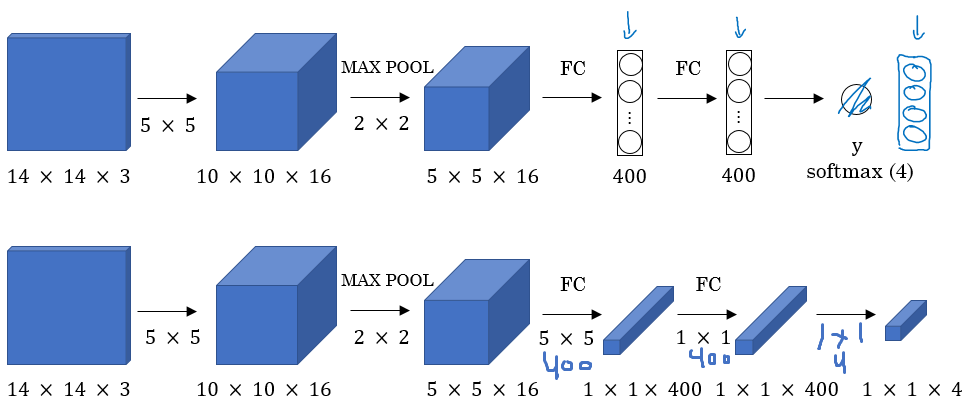
\includegraphics[width=1.0\textwidth]{img/c4/sliding-window.png}
    \caption{Convolutional implementation of sliding windows.}
    \label{sliding-window}
\end{figure}

As you can see in the above image, we turned the FC layer into a Conv layer using a convolution with the width and height of the filter which is the same as the width and height of the input.

The convolution implementation of sliding windows:

\begin{itemize}
    \item First lets consider that the Conv net you trained is like this (Figure \ref{sliding-window2}. No FC all is Conv layers.)
    \begin{figure}[!htbp]
        \centering
        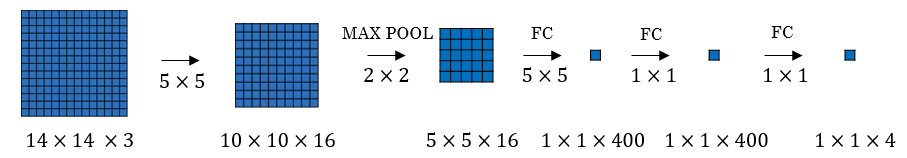
\includegraphics[width=1.0\textwidth]{img/c4/sliding-window2.png}
        \caption{Convolutional implementation of sliding windows (Visualization).}
        \label{sliding-window2}
    \end{figure}
    \item Say now we have a $16\times 16\times 3$ image that we need to apply the sliding windows in. By the normal implementation that has been mentioned in the section before, we would run this Conv net four times each rectangle size will be $14\times 14$.
    \item The convolution implementation will be as follows:
        \begin{figure}[!htbp]
            \centering
            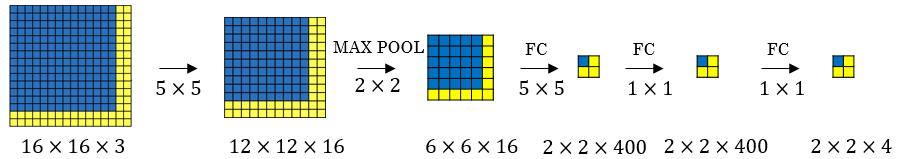
\includegraphics[width=1.0\textwidth]{img/c4/sliding-window3.png}
            \caption{Convolutional implementation of sliding windows (Visualization).}
            \label{sliding-window3}
        \end{figure}
    \item The left cell of the result "blue one" will represent the first sliding window of the normal implementation. The other cells will represent the others.
    \item Its more efficient because it now shares the computations of the four times needed.
\end{itemize}

The weakness of the algorithm is that the position of the rectangle won't be so accurate. Maybe none of the rectangles is exactly on the object you want to recognize (Figure \ref{fail2recognize}).

\begin{figure}[!htbp]
    \centering
    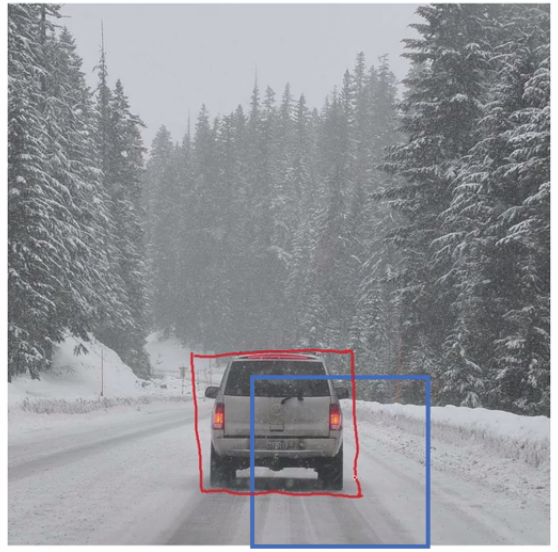
\includegraphics[width=1.0\textwidth, trim={0 0 0 200}, clip]{img/c4/fail2recognize.png}
    \caption{A failure example of convolutional sliding window algorithm.}
    \label{fail2recognize}
\end{figure}

The rectangle in red is what we want while the rectangle in blue is what the algorithm outputs.

\subsubsection{Bounding Box Predictions}
A better algorithm than the convolutional sliding windows in the last section is the YOLO algorithm \cite{redmon2016you}. 

YOLO algorithm (Figure \ref{yolo1}):

\begin{figure}[!htbp]
    % \flushleft
    \centering
    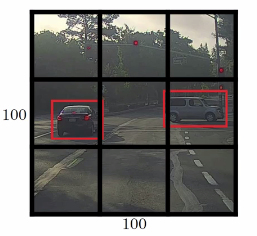
\includegraphics[width=0.5\textwidth, trim={0 0 0 0}, clip]{img/c4/yolo1.png}
    \caption{Example of YOLO algorithm.}
    \label{yolo1}
\end{figure}

\begin{itemize}
    \item Lets say we have an image of $100\times 100$.
    \item Place a $3\times 3$ grid on the image. For more smother results you should use $19\times 19$ for the $100\times100$.
    \item Apply the classification and localization algorithm we discussed in a previous section to each section of the grid. $bx$ and $by$ represent the center point of the object in each grid and will be relative to the box so the range is between 0 and 1 while $bh$ and $bw$ will represent the height and width of the object which can be greater than 1.0 but still a floating point value.
    \item Do everything at once with the convolution sliding window. If Y shape is $1\times8$ as we discussed before then the output of the $100\times 100$ image should be $3\times 3\times 8$ which corresponds to $9$ cell results.
    \item Merging the results using predicted localization mid point.
\end{itemize}

We have a problem if we have found more than one object in one grid box.

One of the best advantages that makes the YOLO algorithm popular is that it has a great speed and a Conv net implementation.

How is YOLO different from other Object detectors? YOLO uses a single CNN network for both classification and localizing the object using bounding boxes.

In the next section we will see some ideas that can make the YOLO algorithm better.

\subsubsection{Intersection Over Union}
Intersection Over Union (IoU) is a function used to evaluate the object detection algorithm. It computes the size of intersection and divide it by the union. More generally, IoU is a measure of the overlap between two bounding boxes.

\subsubsection{Non-Max Suppression}
One of the problems we have addressed in YOLO is that it can detect an object multiple times. Non-max suppression is a way to make sure that YOLO detects the object just one.

For example \ref{nms}:

\begin{figure}[!htbp]
    % \flushleft
    \centering
    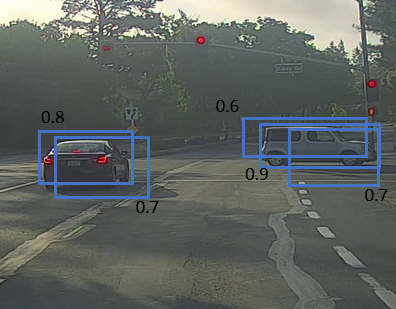
\includegraphics[width=0.5\textwidth, trim={0 0 0 0}, clip]{img/c4/nms.png}
    \caption{Non-max suppression.}
    \label{nms}
\end{figure}

Each car has two or more detections with different probabilities. This came from some of the grids that thinks that this is the center point of the object.

Non-max suppression algorithm:

\begin{itemize}
    \item Lets assume that we are targeting one class as an output class.
    \item Y shape should be $[P_c, b_x, b_y, b_h, b_w]$. Where $P_c$ is the probability if that object occurs.
    \item Discard all boxes with $P_c < 0.6$.
    \item While there are any remaining boxes:
    \begin{itemize}
        \item[i.] Pick the box with the largest $P_c$ output that as a prediction.
        \item[ii.] Discard any remaining box with $IoU > 0.5$ with that box output in the previous step. i.e. any box with high overlap (greater than overlap threshold of 0.5).
    \end{itemize}
\end{itemize}

If there are multiple classes types c you want to detect, you should run the non-max suppression c times, once for every output class.

\subsubsection{Anchor Boxes}
In YOLO, a grid only detects one object. What if a grid cell wants to detect multiple object?

\begin{figure}[!htbp]
    % \flushleft
    \centering
    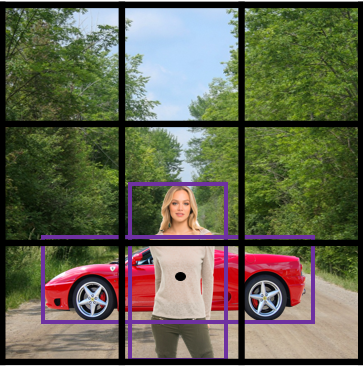
\includegraphics[width=0.5\textwidth, trim={0 0 0 0}, clip]{img/c4/yolo3.png}
    \caption{Example of anchor boxes.}
    \label{anchor}
\end{figure}

As we can see from Figure \ref{anchor}, car and person grid is same here. In practice this actually happens rarely. 

The idea of anchor boxes helps us solving this issue.

If $Y = [Pc, bx, by, bh, bw, c1, c2, c3]$. Then to use two anchor boxes like this:

\begin{itemize}
    \item $Y = [Pc, bx, by, bh, bw, c1, c2, c3, Pc, bx, by, bh, bw, c1, c2, c3]$. We simply have repeated the one anchor Y.
    \item The two anchor boxes you choose should have known shape (Figure \ref{anchor2}):
    \begin{figure}
        \centering
        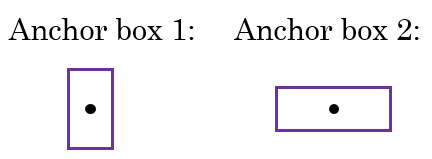
\includegraphics[width=0.6\textwidth]{img/c4/anchor2.png}
        \caption{Visualization of two anchor boxes.}
        \label{anchor2}
    \end{figure}
\end{itemize}

With no anchor box, each object in training image is assigned to grid cell that contains that object's midpoint. With two anchor boxes, each object in training image is assigned to grid cell that contains object's midpoint and anchor box for the grid cell with highest IoU. We suppose that every object detected is similar to an anchor box which has similar shape.

You may have two or more anchor boxes but you should know their shapes.

\begin{itemize}
    \item How do you choose the anchor boxes and people used to just choose them by hand. Maybe five or ten anchor box shapes that spans a variety of shapes that cover the types of objects you seem to detect frequently.
    \item You may also use a k-means algorithm on your dataset to specify that.
\end{itemize}

Anchor boxes allows your algorithm to specialize, means in our case to easily detect wider images or taller ones.

\subsubsection{YOLO Algorithm}
Suppose we need to do object detection for our autonomous driving system. It needs to identify three classes: Pedestrain, Car and Motorcycle.

We decided to choose two anchor boxes, a tall one and a wide one. (Like we said in practice they use five or more anchor boxes hand made or generated using k-means.)

Our labeled Y shape will by $[Ny, HeightOfGrid, WidthOfGrid, 16]$, where $Ny$ is the number of instances and each row is as follows:

\begin{itemize}
    \item $[Pc, bx, by, bh, bw, c1, c2, c3, Pc, bx, by, bh, bw, c1, c2, c3]$
\end{itemize}

Your dataset could be an image with a multiple labels and a rectangle for each label. For example (Figure \ref{yolo2}):

\begin{figure}
    \centering
    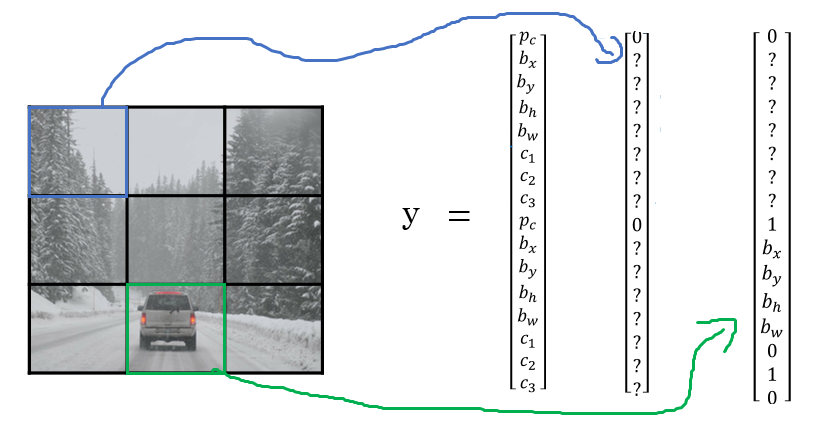
\includegraphics[width=0.8\textwidth]{img/c4/yolo2.png}
    \caption{An extension example of YOLO Ny.}
    \label{yolo2}
\end{figure}

\begin{itemize}
    \item We first initialize all of them to zeors and ?, then for each label and rectangle choose its closest grid point then the shape to fill it and then the best anchor point based on the IoU, so that the shape of Y for one image should be $[HeightOfGrid, WidthOfGrid,16]$.
\end{itemize}

Train the labeled images on a Conv net, you should receive an output of $[HeightOfGrid, WidthOfGrid,16]$ of our case.

To make predictions, run the Conv net on an image and run non-max suppression algorithm for each class you have. In our case, there are 3 classes (Figure \ref{yolo4}). Total number of generated boxes are grid\_width * grid\_height * num\_anchors = $3\times 3 \times 2$. By removing the low probability predictions you should have (Figure \ref{yolo5}). Then get the best probability followed by the IoU filtering (Figure \ref{yolo6}). The details network set up could refer to \href{https://github.com/mbadry1/DeepLearning.ai-Summary/tree/master/4-\%20Convolutional\%20Neural\%20Networks#yolo-algorithm}{Github}.

\begin{figure}[!htbp]
\begin{subfigure}{.33\textwidth}
  \centering
  % include first image
  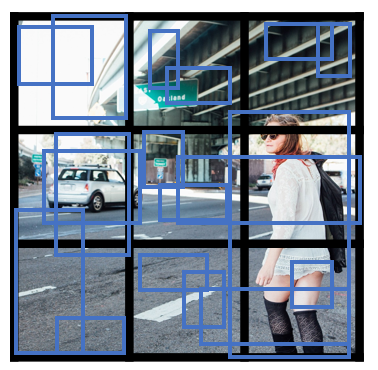
\includegraphics[width=1.0\linewidth]{img/c4/yolo4.png}  
  \caption{Predicted anchor boxes.}
  \label{yolo4}
\end{subfigure}
\begin{subfigure}{.33\textwidth}
  \centering
  % include second image
  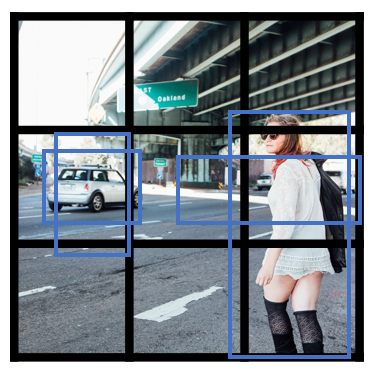
\includegraphics[width=1.0\linewidth]{img/c4/yolo5.png}  
  \caption{Predicted anchor boxes (removing low probability predictions).}
  \label{yolo5}
\end{subfigure}
\begin{subfigure}{.33\textwidth}
  \centering
  % include third image
  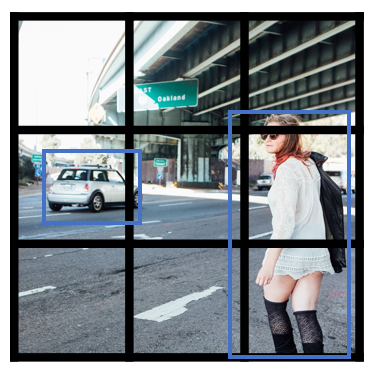
\includegraphics[width=1.0\linewidth]{img/c4/yolo6.png}
  \caption{Predicted anchor boxes (removing low probability predictions and using IoU filtering).}
  \label{yolo6}
\end{subfigure}
\end{figure}

\subsubsection{Region Proposals (R-CNN)}
YOLO is fast but the downside of it is that it process a lot of areas where no objects are presented. R-CNN tries to pick a few windows and run a Conv net (your confident classifier) on top of them.

The algorithm R-CNN \cite{girshick2014rich} uses to pick windows is called a segmentation algorithm. Outputs something like this (Figure \ref{rcnn1}):

\begin{figure}
    \centering
    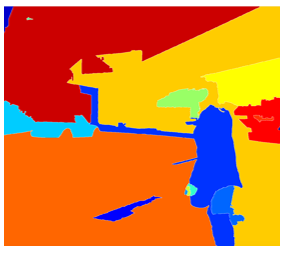
\includegraphics[width=0.6\textwidth]{img/c4/rcnn1.png}
    \caption{Segmentation result by using R-CNN to pick windows.}
    \label{rcnn1}
\end{figure}

If for example the segmentation algorithm produces 2000 blob then we should run our classifier/CNN on top of these blobs.

There has been a lot of work regarding R-CNN tries to make it faster:

\begin{itemize}
    \item R-CNN\cite{girshick2014rich}: Propose regions. Classify proposed regions one at a time. Output label + bounding box. Downside is that it's slow.
    \item Fast R-CNN\cite{girshick2015fast}: Propose regions. Use convolution implementation of sliding windows to classify all the proposed regions.
    \item Faster R-CNN\cite{ren2015faster}: Use convolutional network to propose regions.
    \item Mask R-CNN\cite{he2017mask}.
\end{itemize}

Most of the implementations of faster R-CNN are still slower than YOLO. Andrew Ng thinks that the idea behind YOLO is better than R-CNN because you're able to do all the things in just one stage instead of two stages.


\subsection{Face Recognition}
% \subsection{Special Applications: Face Recognition and Neural Style Transfer}
This section and the next section are aimed at discovering how CNNs can be applied to multiple fields, including art generation and face recognition. Besides, try to implement you own algorithm to generate art and recognize faces. So first we will talke about face recognition.

\subsubsection{What Is Face Recognition?}
Face recognition system identifies a person's face. It can work on both images or videos.

Face verification vs. face recognition:

\begin{itemize}
    \item Verification:
    \begin{itemize}
        \item Input: image, name/ID. (1:1)
        \item Output: whether the input image is that of the claimed person.
        \item "Is this the claimed person?"
    \end{itemize}
    \item Recognition:
    \begin{itemize}
        \item Has a database of K persons and get an input image.
        \item Output ID if the image is any of the K persons (or not recognized).
        \item "Who is this person?"
    \end{itemize}
\end{itemize}

We can use a face verification system to make a face recognition system. The accuracy of the verification system has to be high (around 99.9\% or more) to be use accurately within a recognition system because the recognition system accuracy will be less than the verification system given K persons.

\subsubsection{One-Shot Learning}
One of the face recognition challenges is to solve one shot learning problem.

One Shot Learning: A recognition system is able to recognize a person, learning from one image.

Historically deep learning doesn't work well with a small number of data.

Instead to make this work, we will learn a \textbf{similarity function}:
\begin{itemize}
    \item d(img1, img2) = degree of difference between images.
    \item We want d result to be low in case of the same faces.
    \item We use $\tau$ as a threshold for d: if d(img1, img2) $\leq \tau$, then the faces are the same.
\end{itemize}

Similarity function helps us solving the one shot learning. Also its robust to new inputs.

\subsubsection{Siamese Network}
We will implement the similarity function using a type of NNs called Siamese Network \cite{koch2015siamese} in which we can pass multiple inputs to the two or more networks with the same architecture and parameters.

Siamese network architecture is as the following (Figure \ref{siamese}):

\begin{figure}[!htbp]
    \centering
    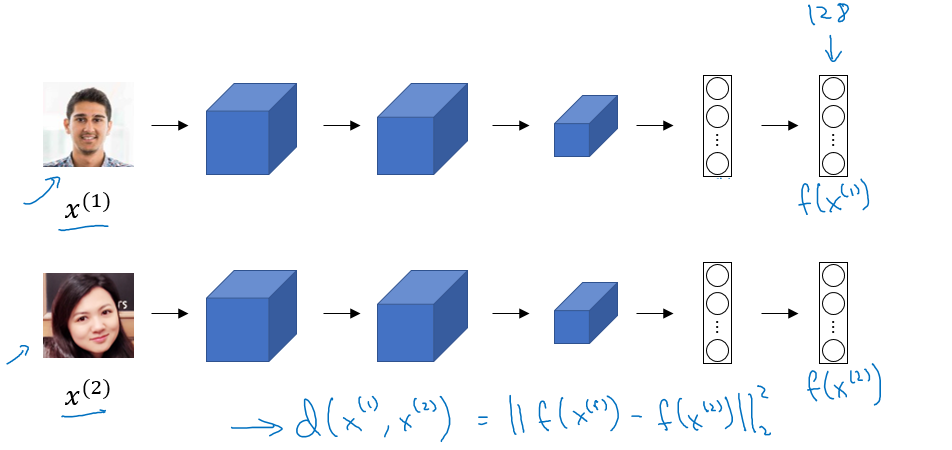
\includegraphics[width=1.0\textwidth]{img/c4/siamese.png}
    \caption{Siamese network.}
    \label{siamese}
\end{figure}

We make 2 identical ConvNets which encoders an input image into a vector. In the above image the vector shape is (128,). 

The loss function will be $d(x1, x2) = ||f(x1) - f(x2)||^2$.

If x1 and x2 are the same person, we want d to be low. If they are different persons, we want d to be high.

\subsubsection{Triplet Loss}
Triplet loss is one of the loss functions we can use to solve the similarity distance in a Siamese Network.

Our learning objective in the triplet loss function is to get the distance between an \textbf{anchor} image and a positive or a negative image (positive means same person, while negative means different person).

The triplet name came from that we are comparing an anchor A with a positive P and a negative N image.

Formally we want:

\begin{itemize}
    \item Positive distance to be less than negative distance: $||f(A)-f(P)||^2 \leq ||f(A) - f(N)||^2$.
    \item Then $||f(A)-f(P)||^2 - ||f(A) - f(N)||^2 \leq 0$.
    \item To make sure the NN won't get an output of zeros easily: $||f(A)-f(P)||^2 - ||f(A) - f(N)||^2 \leq -\alpha$. $\alpha$ is a small number. Sometimes its called the margin.
    \item Then $||f(A)-f(P)||^2 - ||f(A) - f(N)||^2 + \alpha \leq 0$. 
\end{itemize}

Final loss function:
\begin{itemize}
    \item Given 3 images (A, P, N)
    \item $L(A, P, N) = \max (||f(A)-f(P)||^2 - ||f(A) - f(N)||^2 + \alpha, 0)$.
    \item $J = \sum(L(A[i], P[i], N[i]))$ for all triplets of images.
\end{itemize}

You need multiple images of the same person in your dataset. Then get some triplets out of your dataset. Dataset should be big enough.

Choosing the triplets A, P, N:

\begin{itemize}
    \item During training, if A, P, N are chosen randomly (subject to A and P are the same and A and N aren't the same), then one of the problems is the following constrain is easily satisfied ($d(A, P) + \alpha \leq d(A, N)$). So the NN won't learn much.
    \item What we want to do is to choose triplets that are hard to train on. So for all the triplets we want the above equation to be satisfied. Details are in FaceNet\cite{schroff2015facenet}.
\end{itemize}

\subsubsection{Face Verification and Binary Classification}
Triplet loss is one way to learn the parameters of a ConvNet for face recognition. However, there's another way to learn these parameters as a straight binary classification problem.

Learning the similarity function another way\cite{taigman2014deepface} (Figure \ref{triplet-loss}):

\begin{figure}[!htbp]
    \centering
    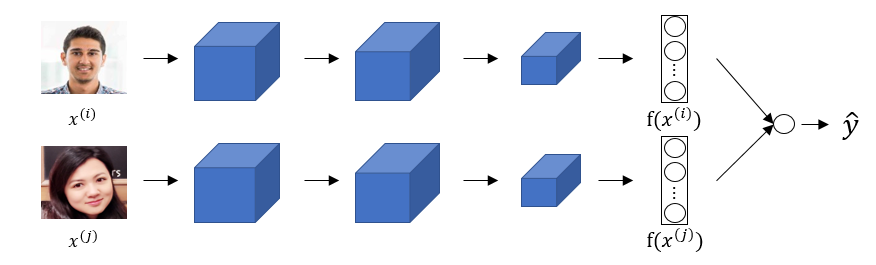
\includegraphics[width=1.0\textwidth]{img/c4/triplet-loss.png}
    \caption{Learning the similarity function in one network.}
    \label{triplet-loss}
\end{figure}

\begin{itemize}
    \item The final layer is a sigmoid layer.
    \item $\hat{Y} = w_{ij} sigmoid (f(x_i) - f(x_j)) + b$, where the substraction is the Manhattan distance between $f(x_i)$ and $(f(x_j)$.
    \item Some other similarities can be Euclidean distance similarity.
\end{itemize}

A good performance/deployment trick:
\begin{itemize}
    \item Pre-compute all the images that you're using as a comparison to the vector $f(x_j)$.
    \item When a new image that needs to be compared, get its vector $f(x_i)$ then put it with all the pre-computed vectors and pass it to the sigmoid function.
\end{itemize}

This version works quite as well as the triplet loss function.

\subsection{Neural Style Transfer}
\subsubsection{What Is Neural Style Transfer?}
Neural style transfer takes a content image $c$ and a style image $s$ and generates the content image $g$ with the style of style image. e.g. Figure \ref{style-transfer}.

\begin{figure}[!htbp]
    \centering
    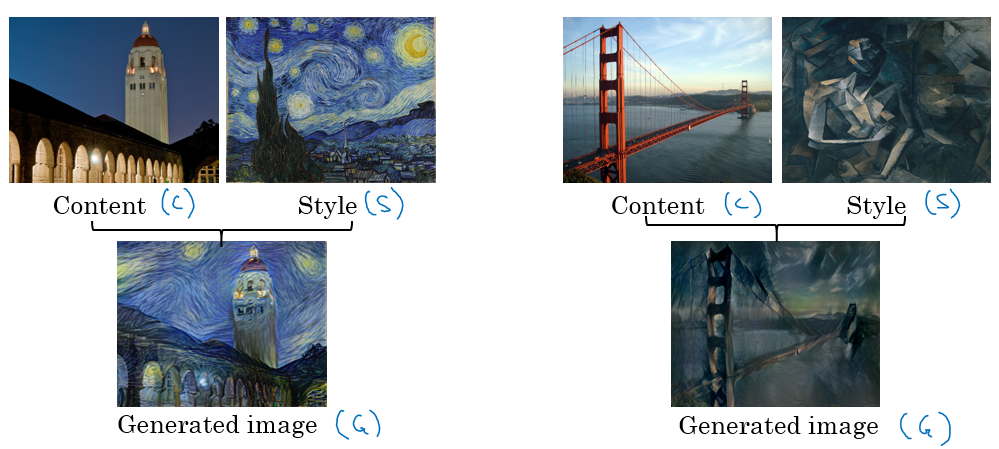
\includegraphics[width=1.0\textwidth]{img/c4/style-transfer.png}
    \caption{Examples of neural style transfer.}
    \label{style-transfer}  
\end{figure}

In order to implement this you need to look at the features extracted by the ConvNet at the shallower and deeper layers.

It uses a previously trained convolutional network like VGG, and builds on top of that. The idea of using a network trained on a different task and applying it to a new task is called transfer learning.

\subsubsection{What Is Deep ConvNets Learning?}
Visualizing what a deep network is learning. Firstly, give this AlexNet like ConvNet (Figure \ref{visualize-convs}).

\begin{figure}[!htbp]
    \centering
    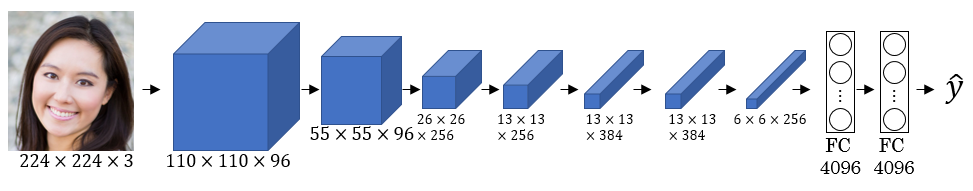
\includegraphics[width=1.0\textwidth]{img/c4/visualize-convnets.png}
    \caption{AlexNet like ConvNet.}
    \label{visualize-convs}  
\end{figure}

Pick a unit in layer l. Find the nine image patches that maximize the unit's activation. Notice that a hidden unit in layer 1 will see relatively small portion of NN, so if you plotted it it will match a msall image in the shallower layers while it will get larger image in deeper layers.

Repeating for other units and layers.

It turns out that layer 1 is learning the low level representations like colors and edges.

You will find out that deeper layers are learning more complex representations\cite{zeiler2014visualizing} (Figure \ref{visualize-convs2}).

\begin{figure}[!htbp]
    \centering
    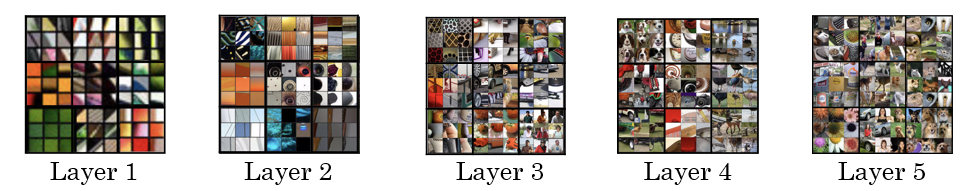
\includegraphics[width=1.0\textwidth]{img/c4/visualize-convnets2.png}
    \caption{Visualization of ConvNets.}
    \label{visualize-convs2}  
\end{figure}

A good explanation on how to get receptive field given a layer\footnote{https://medium.com/mlreview/a-guide-to-receptive-field-arithmetic-for-convolutional-neural-networks-e0f514068807} (Figure \ref{receptivefield}):

\begin{figure}[!htbp]
    \centering
    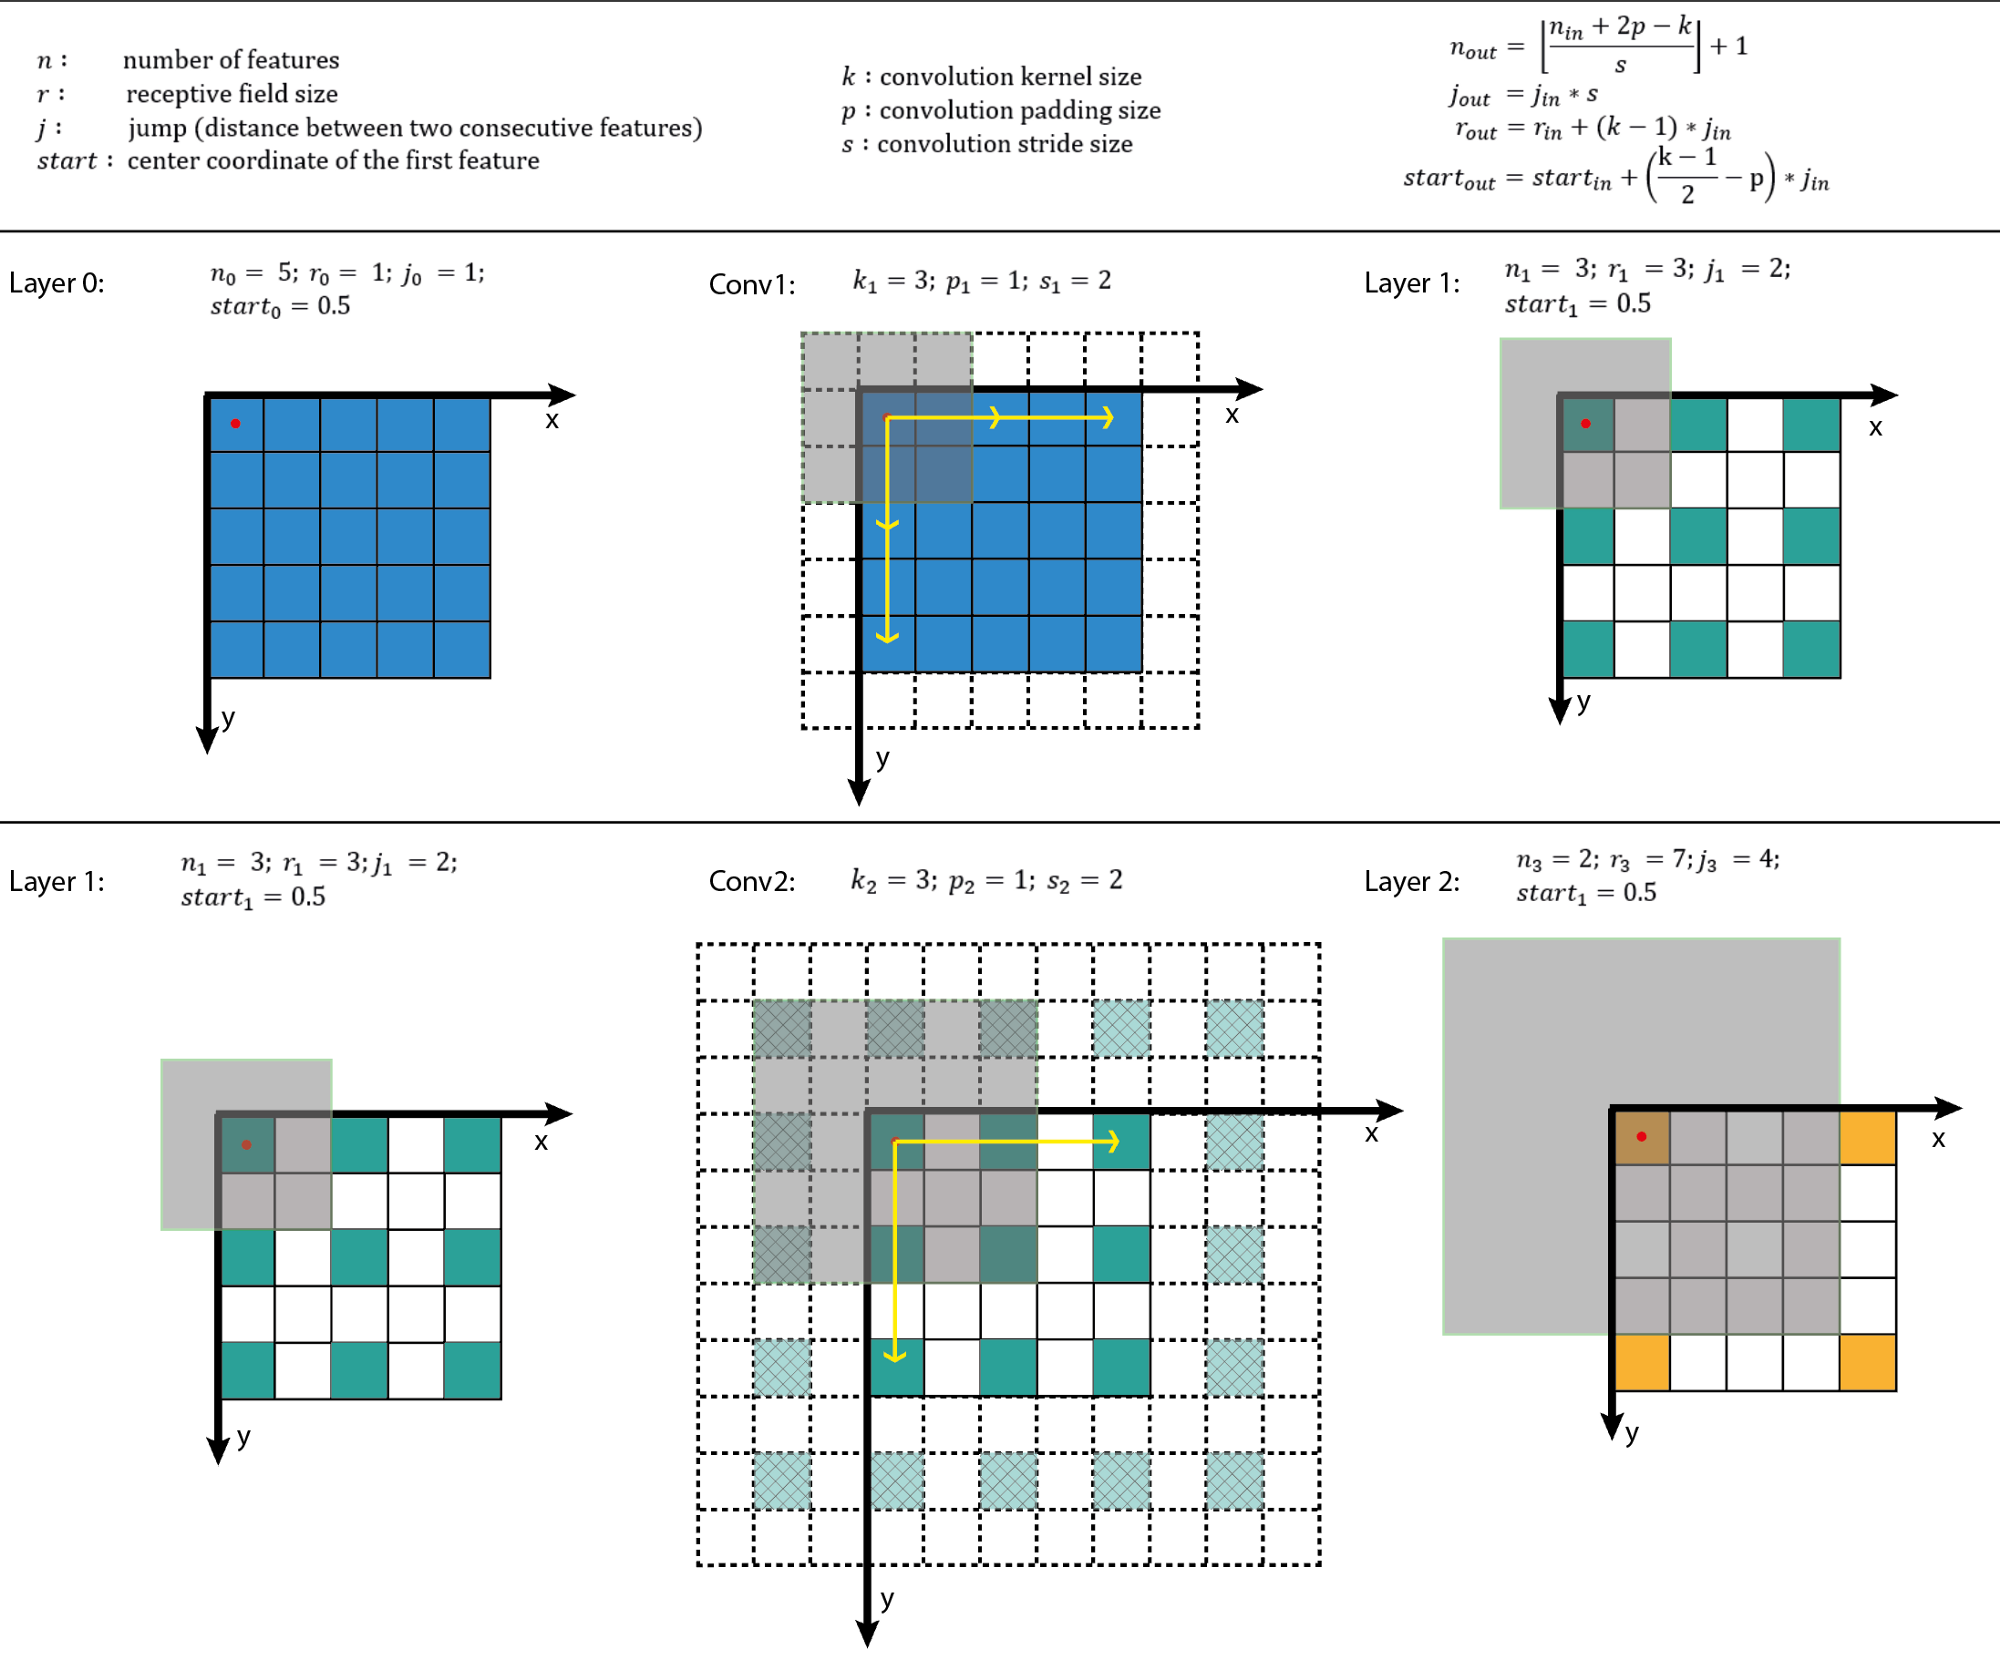
\includegraphics[width=1.0\textwidth]{img/c4/receptiveField.png}
    \caption{An explanation of how to get receptive field.}
    \label{receptivefield}  
\end{figure}  

% not very familiar with how to calculate receptive field.

\subsubsection{Cost Function}
We will define a cost function for the generated image that measures how good it is.

Given a content image C, a style image S, and a generated image G:
\begin{itemize}
    \item $J(G) = \alpha J(C, G) + \beta J(S, G)$
    \item $J(C, G)$ measures how similar is the generated image to the content image.
    \item $J(S, G)$ measures how similar is the generated image to the style image.
    \item $\alpha$ and $\beta$ are relative weighting to the similarity and these are hyperparameters.
\end{itemize}

Find the generated image G:

\begin{itemize}
    \item[i.] Initialize G randomly.
    \item[ii.] Use gradient descent to minimize $J(G)$. $G = G - dG$. We compute the gradient image and use gradient descent to minimize the cost function.
\end{itemize}

The iterations might be as following image:

To generate by using the following (Figure \ref{cgimage}):

\begin{figure}[!htbp]
    \centering
    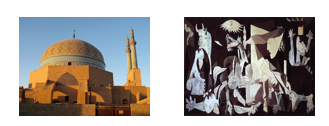
\includegraphics[width=1.0\textwidth]{img/c4/cgimage.png}
    \caption{Provided content image C and style image G.}
    \label{cgimage}  
\end{figure}  

You will go through this (Figure \ref{stagedG}):
\begin{figure}[!htbp]
    \centering
    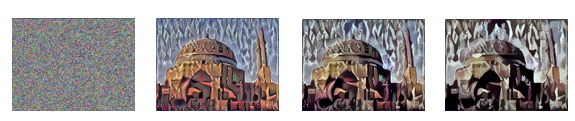
\includegraphics[width=1.0\textwidth]{img/c4/stagedG.png}
    \caption{Staged pictures of generated image G.}
    \label{stagedG}  
\end{figure}  

\subsubsection{Content Cost Function}
In the previous section we showed that we need a cost function for the content image and the style image to measure how similar is them to each other.

Say you use hidden layer $l$ to compute content cost. If we choose $l$ to be small (like layer 1), we will force the network to get similar output to the original content image. In practice $l$ is not too shallow or not too deep but in the middle.

Use pre-trained ConvNet like VGG network.

Let $a(C)[l]$ and $a(G)[l]$ be the activation of layer $l$ on the images.

If $a(C)[l]$ and $a(G)[l]$ are similar then they will have the same content:

\begin{equation}
    J(C, G) at layer l = \frac{1}{2} ||a(C)[l] - a(G)[l]||^2
\end{equation}

\subsubsection{Style Cost Function}
Meaning of the \textbf{style} of an image:

\begin{itemize}
    \item Say you're using layer $l$'s activation to measure \textbf{style}.
    \item Define style as correlation between activations across channels. That means given an activation like Figure \ref{style-cost}. How correlate is the orange channel with the yellow channel?
    \begin{figure}[!htbp]
    \centering
    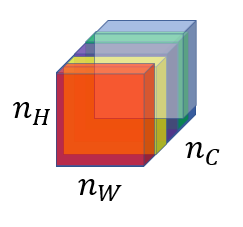
\includegraphics[width=0.4\textwidth]{img/c4/style-cost.png}
    \caption{Illustration of image style.}
    \label{style-cost}  
    \end{figure}  
    \item Correlated means if a value appeared in a specific channel a specific value will appear too (depend on each other). While uncorrelated means if a value appeared in a specific channel doesn't mean that the another value will appear (not depend on each other). The correlation tells you how a components might occur or not occur together in the same image.
\end{itemize}

The correlation of style image channels should appear in the generated image channels. 

Style matrix (Gram matrix):

\begin{itemize}
    \item Let $a(l)[i, j, k]$ be the activation at layer $l$ with $i=H, j=W, k=C$.
    \item Also $G(l)(s)$ is the matrix of shape $n_C(l)\times n_C(l)$ (We call this matrix style matrix or Gram matrix). In this matrix, each cell will tell us how correlated is a channel to another channel.
    \begin{equation}
        \begin{aligned}
        G_{kk'}^{[l](S)} &= \sum^{n_H^{l}}_{i=1}\sum^{n_W^{[l}}_{j=1} a_{ijk}^{[l](S)} a_{ijk'}^{[l](S)}\\
        G_{kk'}^{[l](G)} &= \sum^{n_H^{l}}_{i=1}\sum^{n_W^{[l}}_{j=1} a_{ijk}^{[l](G)} a_{ijk'}^{[l](G)}\\
        \end{aligned}
    \end{equation}
\end{itemize}

% Not too familiar with this equations.

Steps to be made if you want to create a tensorflow model for neural style transfer.

\begin{itemize}
    \item[i.] Create an Interactive Session.
    \item[ii.] Load the content image, load the style image
    \item[iii.] Randomly initialize the image to be generated.
    \item[iv.] Load the VGG16 model
    \item[v.] Build the TensorFlow graph: 1) Run the content image through the VGG16 model and compute the content cost; 2) Run the style image through the VGG16 model and compute the style cost; 3) Compute the total cost; 4) Define the optimizer and the learning rate.
    \item[vi.] Initialize the TensorFlow graph and run it for a large number of iterations, updating the generated image at every step.
\end{itemize}

\subsubsection{Keras Tutorial}
To train and test a model in Keras there are four steps:

\begin{itemize}
    \item[i.] Create the model.
    \item[ii.] Compile the model by calling \textit{model.compile(optimizer = "...", loss = "...", metrics = ["accuracy"])}.
    \item[iii.] Train the model on train data by calling \textit{model.fit(x = ..., y = ..., epochs = ..., batch\_size = ...)}. (We can add a validation set while training too.)
    \item Test the model on test data by calling \textit{model.evaluate(x = ..., y = ...)}.
\end{itemize}

Summarize of steps in Keras: Create $\to$ Compile $\to$ Fit/Train $\to$ Evaluate/Test.

Model.summary() gives a lot of useful informations regarding your model including each layers inputs, outputs, and number of parameters at each layer.

To choose the Keras backend you should go to \$HOME/.keras/keras.json and change the file to the desired backend like Theano or Tensorflow or whatever backend you want.

After you create the model you can run it in a tensorflow session without compiling, training, and testing capabilities.

You can save your model with model\_save and load your model using model\_load This will save your whole trained model to disk with the trained weights.